\documentclass[12pt,a4paper]{article}
\usepackage{fontspec}
\usepackage{amsmath,amssymb,amsthm}
\usepackage{array,booktabs,longtable}
\usepackage[margin=2.3cm,headheight=15pt]{geometry}
\usepackage{enumitem}
\usepackage{xcolor}
\usepackage{titlesec}
\usepackage{mdframed}
\usepackage{fancyhdr}
\usepackage{graphicx}
\usepackage{float}
\usepackage{listings}
\usepackage[hidelinks]{hyperref}

\setmainfont{Times New Roman}
\setsansfont{Arial}[Scale=0.92]
\setmonofont{Courier New}[Scale=0.92]

\definecolor{dnavy}{HTML}{123A6B}
\definecolor{dred}{HTML}{B02418}
\definecolor{dgray}{HTML}{F2F4F7}
\definecolor{dwarn}{HTML}{FFF4D6}

\titleformat{\section}{\sffamily\large\bfseries\color{dnavy}}{\thesection.}{0.6em}{}
\titleformat{\subsection}{\sffamily\normalsize\bfseries\color{dred}}{\thesubsection}{0.6em}{}
\titlespacing{\section}{0pt}{14pt}{6pt}
\titlespacing{\subsection}{0pt}{10pt}{4pt}

\newmdenv[backgroundcolor=dgray,linewidth=0pt,skipabove=6pt,skipbelow=6pt,
innertopmargin=6pt,innerbottommargin=6pt]{note}
\newmdenv[backgroundcolor=dwarn,linewidth=0pt,skipabove=6pt,skipbelow=6pt,
innertopmargin=6pt,innerbottommargin=6pt]{xacnhan}
\setlist[enumerate]{itemsep=2pt,topsep=3pt}
\setlist[itemize]{itemsep=2pt,topsep=3pt}

\lstset{basicstyle=\ttfamily\small,columns=fullflexible,keepspaces=true,frame=single,
  rulecolor=\color{black!20},backgroundcolor=\color{dgray},numbers=left,numberstyle=\tiny\color{gray},
  xleftmargin=1.5em,breaklines=true,showstringspaces=false}

\pagestyle{fancy}\fancyhf{}
\lhead{\small\sffamily CS112 -- Phân tích \& Thiết kế thuật toán}
\rhead{\small\sffamily Bài tập lớn -- Đường đi an toàn}
\cfoot{\small\thepage}
\renewcommand{\headrulewidth}{0.4pt}

\begin{document}

% ==================== TRANG BÌA ====================
\begin{titlepage}
\centering
\vspace*{0.6cm}
{\large ĐẠI HỌC QUỐC GIA THÀNH PHỐ HỒ CHÍ MINH}\\[4pt]
{\large\bfseries TRƯỜNG ĐẠI HỌC CÔNG NGHỆ THÔNG TIN}\\[4pt]
{\large KHOA KHOA HỌC MÁY TÍNH}\\[1.2cm]
\rule{\linewidth}{1pt}\\[10pt]
{\Large\bfseries\color{dnavy} BÀI TẬP LỚN -- DEMO CÓ GIAO DIỆN}\\[14pt]
{\LARGE\bfseries ĐƯỜNG ĐI AN TOÀN}\\[10pt]
{\large\itshape Trực quan hóa thuật toán Quy hoạch động đếm đường đi trên lưới}\\[10pt]
\rule{\linewidth}{1pt}\\[1.4cm]
\begin{tabular}{@{}>{\bfseries}l l@{}}
Tên môn học: & Phân tích \& Thiết kế thuật toán \\[6pt]
Mã lớp: & CS112.2026.TX \\[6pt]
Giảng viên: & Huỳnh Thị Thanh Thương \\[6pt]
Sinh viên: & Đinh Văn Huy -- 25730032 \\[6pt]
Hình thức: & Cá nhân \\[6pt]
Bài toán chọn: & ``Đường đi an toàn'' (WeCode -- nhóm Dynamic Programming)\\
\end{tabular}
\vfill
{\large TP. Hồ Chí Minh, tháng 10 năm 2026}
\end{titlepage}

\tableofcontents
\newpage

% =====================================================
\section{Yêu cầu của bài tập lớn}
Theo yêu cầu cô giao ở Buổi 8 (đầu buổi, khoảng phút 12--22; nhắc lại cuối buổi), sinh viên chọn một bài toán đã học hoặc đã làm trên WeCode và xây dựng một \textbf{demo có giao diện}: có ô nhập dữ liệu, khung hiển thị kết quả, minh họa trực quan quá trình giải; được phép dùng AI. Sản phẩm nộp gồm ba phần:
\begin{enumerate}
  \item \textbf{Source code} của sản phẩm (thư mục \texttt{app/}, \texttt{solution/}, \texttt{tests/}).
  \item \textbf{Video} quay quá trình chạy thử (\texttt{video/demo.mp4}).
  \item \textbf{Report} (tài liệu này) tường thuật lại toàn bộ quy trình: tìm hiểu, dùng AI nào, prompt ra sao, thuật toán do ai đề xuất và kiểm chứng thế nào.
\end{enumerate}
Em chọn bài \textbf{Đường đi an toàn} vì bài có lời giải quy hoạch động (QHĐ) ngắn gọn nhưng rất phù hợp để minh họa: mỗi ô của bảng là một bài toán con, và việc ``điền bảng'' có thể diễn ra trực tiếp trên bản đồ. Mục tiêu đặt ra không chỉ là cho ra đáp án, mà là giúp \textbf{người mới học hiểu được vì sao công thức truy hồi đúng}.

% =====================================================
\section{Phát biểu bài toán}
\subsection*{Đề bài (tóm tắt)}
Bản đồ làng đại học kích thước $n\times n$; một số ô có chốt cảnh sát giao thông. Tấn Lưu đi từ KTX khu B ở ô $[1,1]$ (góc trái trên) tới UIT ở ô $[n,n]$ (góc phải dưới), mỗi bước chỉ được \textbf{sang phải} hoặc \textbf{xuống dưới}. Đếm số con đường không đi qua chốt nào, lấy dư cho $10^9+7$.

\subsection*{Input}
\begin{itemize}
  \item $n$: số nguyên, $1 \le n \le 1000$ -- kích thước bản đồ.
  \item $A = (a_{ij})_{n\times n}$, $a_{ij} \in \{\texttt{.},\texttt{*}\}$ -- bản đồ; $a_{ij}=\texttt{*}$ nghĩa là ô $(i,j)$ có chốt, $a_{ij}=\texttt{.}$ là ô trống. Cho dưới dạng $n$ dòng, mỗi dòng đúng $n$ ký tự.
\end{itemize}
\subsection*{Output}
\begin{itemize}
  \item $R$: số nguyên, $0 \le R < 10^9+7$, với $R = |\mathcal P| \bmod (10^9+7)$, trong đó $\mathcal P$ là tập các dãy ô $(1,1)=c_0,c_1,\dots,c_{2n-2}=(n,n)$ sao cho mỗi $c_{k+1}$ là ô bên phải hoặc ô phía dưới của $c_k$, và $a_{c_k} = \texttt{.}$ với mọi $k$.
\end{itemize}

\begin{note}
\textbf{Ví dụ trong đề (hình minh họa).} Với
\texttt{n = 4}, bản đồ \texttt{....\,/\,.*..\,/\,...*\,/\,*...} thì đáp án là \textbf{3}.
\end{note}

% =====================================================
\section{Thiết kế thuật toán}
\subsection{Vì sao không vét cạn?}
Khi không có chốt, mỗi đường gồm $n-1$ bước xuống và $n-1$ bước sang phải theo thứ tự tùy ý, nên có $\binom{2n-2}{n-1}$ đường. Với $n=1000$ con số này cỡ $10^{598}$ -- liệt kê từng đường là bất khả thi. Tuy nhiên rất nhiều đường \emph{dùng chung đoạn đầu}: số cách đi tới một ô chỉ phụ thuộc vào ô đó chứ không phụ thuộc vào phần đường còn lại. Đây chính là tính chất \textbf{bài toán con gối nhau} -- dấu hiệu dùng quy hoạch động.

\subsection{Trạng thái và công thức truy hồi}
Gọi $dp[i][j]$ là số đường an toàn từ $(1,1)$ tới $(i,j)$. Quy ước $dp[i][j]=0$ nếu $i=0$ hoặc $j=0$ (ngoài bản đồ).
\[
dp[i][j] =
\begin{cases}
0 & \text{nếu } a_{ij}=\texttt{*},\\
1 & \text{nếu } (i,j)=(1,1) \text{ và } a_{11}=\texttt{.},\\
\big(dp[i-1][j] + dp[i][j-1]\big) \bmod (10^9+7) & \text{ngược lại.}
\end{cases}
\]
Đáp án: $dp[n][n]$.

\subsection{Chứng minh tính đúng đắn}
Xét ô trống $(i,j)\ne(1,1)$. Mọi đường an toàn tới $(i,j)$ có \emph{bước cuối} hoặc là bước xuống từ $(i-1,j)$, hoặc là bước sang phải từ $(i,j-1)$ -- không còn khả năng nào khác vì chỉ được đi phải/xuống. Hai nhóm này \textbf{rời nhau} (bước cuối khác nhau) và \textbf{phủ hết} mọi đường. Bỏ bước cuối của một đường thuộc nhóm thứ nhất ta được đúng một đường an toàn tới $(i-1,j)$ và ngược lại (song ánh), tương tự cho nhóm thứ hai. Theo quy tắc cộng, số đường tới $(i,j)$ bằng $dp[i-1][j]+dp[i][j-1]$. Ô có chốt không thể nằm trên đường an toàn nên $dp=0$. Trường hợp cơ sở $(1,1)$: có đúng một đường (đường rỗng).
Bằng quy nạp theo thứ tự duyệt (hàng tăng dần, trong mỗi hàng cột tăng dần) -- khi tính $(i,j)$ thì $(i-1,j)$ và $(i,j-1)$ đã được tính đúng -- ta có mọi $dp[i][j]$ đều đúng.

Việc lấy dư sau mỗi phép cộng là hợp lệ vì $(x+y)\bmod p = \big((x\bmod p)+(y\bmod p)\big)\bmod p$.

\subsection{Mã giả}
\begin{lstlisting}[numbers=left]
SafePaths(n, A):
    P <- 10^9 + 7
    dp[1..n] <- [1, 0, 0, ..., 0]
    for i <- 1 to n:
        for j <- 1 to n:
            if A[i][j] = '*':   dp[j] <- 0
            else if j > 1:      dp[j] <- (dp[j] + dp[j-1]) mod P
    return dp[n]
\end{lstlisting}
\textbf{Nén bộ nhớ.} Hàng $i$ chỉ phụ thuộc hàng $i-1$. Dùng một mảng $dp[1..n]$: ngay trước khi cập nhật, $dp[j]$ vẫn giữ giá trị của \emph{ô phía trên} $(i-1,j)$, còn $dp[j-1]$ vừa được cập nhật nên là \emph{ô bên trái} $(i,j-1)$. Với $j=1$ chỉ có ô phía trên nên giữ nguyên $dp[1]$ (trừ khi gặp chốt). Ô $(1,1)$ được khởi tạo bằng 1 trước vòng lặp; nếu $(1,1)$ là chốt, lệnh ở dòng 6 đưa nó về 0 -- đúng.

\subsection{Độ phức tạp}
Mỗi ô được xử lý đúng một lần với $O(1)$ phép tính: $T(n) = \sum_{i=1}^{n}\sum_{j=1}^{n} c = c\,n^2 \in \Theta(n^2)$. Với $n=1000$ là $10^6$ phép tính. Bộ nhớ phụ $\Theta(n)$ cho mảng $dp$ (không tính bộ nhớ đọc input -- lời giải đọc và xử lý từng dòng nên cũng chỉ cần $\Theta(n)$).

\subsection{Ví dụ chạy tay (ví dụ trong đề)}
\begin{center}
\begin{tabular}{c|cccc}
$dp$ & 1 & 2 & 3 & 4\\\hline
1 & 1 & 1 & 1 & 1\\
2 & 1 & \textbf{0}\,(*) & 1 & 2\\
3 & 1 & 1 & 2 & \textbf{0}\,(*)\\
4 & \textbf{0}\,(*) & 1 & 3 & \textbf{3}\\
\end{tabular}
\end{center}
Chẳng hạn $dp[4][4] = dp[3][4] + dp[4][3] = 0 + 3 = 3$ -- khớp đáp án.

% =====================================================
\section{Kiểm chứng lời giải}
Thuật toán được AI đề xuất (xem mục~\ref{sec:quytrinh}), vì vậy em không tin ngay mà kiểm chứng bằng ba cách:
\begin{enumerate}
  \item \textbf{Chạy tay} ví dụ trong đề (bảng ở trên) -- ra 3, đúng.
  \item \textbf{Đối chiếu với vét cạn} (\texttt{tests/run\_tests.py}): một hàm liệt kê từng đường đi bằng ngăn xếp (không nhớ, không dùng công thức QHĐ) làm ``đáp án chuẩn''. Chạy trên 307 bản đồ: ví dụ trong đề, 6 trường hợp biên ($n=1$, chốt ở KTX, chốt ở UIT, đường chéo bị chặn,\dots) và 300 bản đồ ngẫu nhiên $n\le 6$ với mật độ chốt 0\%--70\%. Cả lời giải Python lẫn lõi JavaScript của giao diện web đều cho kết quả trùng khớp \textbf{307/307}.
  \item \textbf{Test lớn và phép lấy dư:} với $n=1000$ không có chốt, đáp án phải là $\binom{1998}{999} \bmod (10^9+7) = 965\,601\,742$ (tính độc lập bằng \texttt{math.comb} của Python); cả hai bản cài đặt đều ra đúng số này. Thời gian: Python $\approx 0{,}14$\,s, JavaScript $\approx 0{,}06$\,s (đã gồm khởi động trình thông dịch).
\end{enumerate}
Ngoài ra bộ test còn kiểm tra 7 input sai (rỗng, $n$ không phải số, $n=0$, $n=1001$, thiếu dòng, ký tự lạ, dòng dài sai) -- giao diện từ chối cả 7.

\begin{xacnhan}
\textbf{[Cần sinh viên xác nhận trước khi nộp]} Lời giải Python ở Phụ lục là bản em đã nộp trên WeCode; trạng thái chấm trên WeCode: \underline{\hspace{4cm}} (ví dụ: Accepted 100/100).
\end{xacnhan}

% =====================================================
\section{Sản phẩm: giao diện trực quan hóa}
\subsection{Công nghệ và cách chạy}
Ứng dụng web tĩnh: HTML + CSS + JavaScript thuần, không cần cài đặt hay build. Lõi thuật toán nằm riêng trong \texttt{app/core.js} để dùng chung cho trình duyệt và cho bộ test bằng Node.js.
\begin{itemize}
  \item Chạy: mở \texttt{app/index.html} bằng trình duyệt, hoặc \texttt{python3 -m http.server -d app} rồi vào \texttt{http://localhost:8000}.
  \item Kiểm thử: \texttt{python3 tests/run\_tests.py}.
\end{itemize}

\subsection{Các chức năng chính}
\begin{enumerate}
  \item \textbf{Nhập dữ liệu} đúng định dạng WeCode (ô văn bản); 4 ví dụ có sẵn; \textbf{sinh bản đồ ngẫu nhiên} với $n$ và mật độ chốt tùy chọn; \textbf{bấm trực tiếp lên lưới} để thêm/bỏ chốt.
  \item \textbf{Kiểm tra input đầy đủ}: $n$ không phải số nguyên, $n$ ngoài $[1,1000]$, sai số dòng, dòng sai độ dài, ký tự khác \texttt{.}/\texttt{*} -- báo lỗi kèm số dòng, hàng, cột.
  \item \textbf{Minh họa từng bước}: điền bảng $dp$ theo đúng thứ tự duyệt; ô đang tính tô vàng, ô phía trên tô tím, ô bên trái tô xanh, kèm mũi tên; khung giải thích ghi rõ công thức với số cụ thể, ví dụ $dp[3][2] = dp[2][2] + dp[3][1] = 0 + 1 = 1$; mã giả tô sáng dòng đang thực thi; nhật ký các phép tính.
  \item \textbf{Điều khiển}: chạy/dừng, tiến/lùi từng bước, về đầu/tới cuối, chỉnh tốc độ; phím tắt Space, $\leftarrow$, $\rightarrow$, Home, End.
  \item \textbf{Hai chế độ xem}: bảng 2 chiều $dp[i][j]$ (dễ hiểu) và mảng 1 chiều $dp[j]$ -- đúng như code nộp WeCode, cho thấy vì sao nén bộ nhớ vẫn đúng.
  \item \textbf{Kết quả}: đáp án mod $10^9+7$, \emph{số đường thật} (số nguyên lớn, BigInt) để thấy vì sao phải lấy dư, thời gian chạy; vẽ ngẫu nhiên một đường an toàn; làm mờ các ô không nằm trên đường an toàn nào.
  \item \textbf{Lưới lớn} ($n>16$, tới $1000$): không hoạt hình từng ô mà hiển thị bản đồ nhiệt (màu theo $\log$ số đường tới mỗi ô) cùng kết quả.
  \item \textbf{Song ngữ} Việt/Anh, giao diện sáng/tối, dùng được trên điện thoại.
\end{enumerate}

\begin{figure}[H]\centering
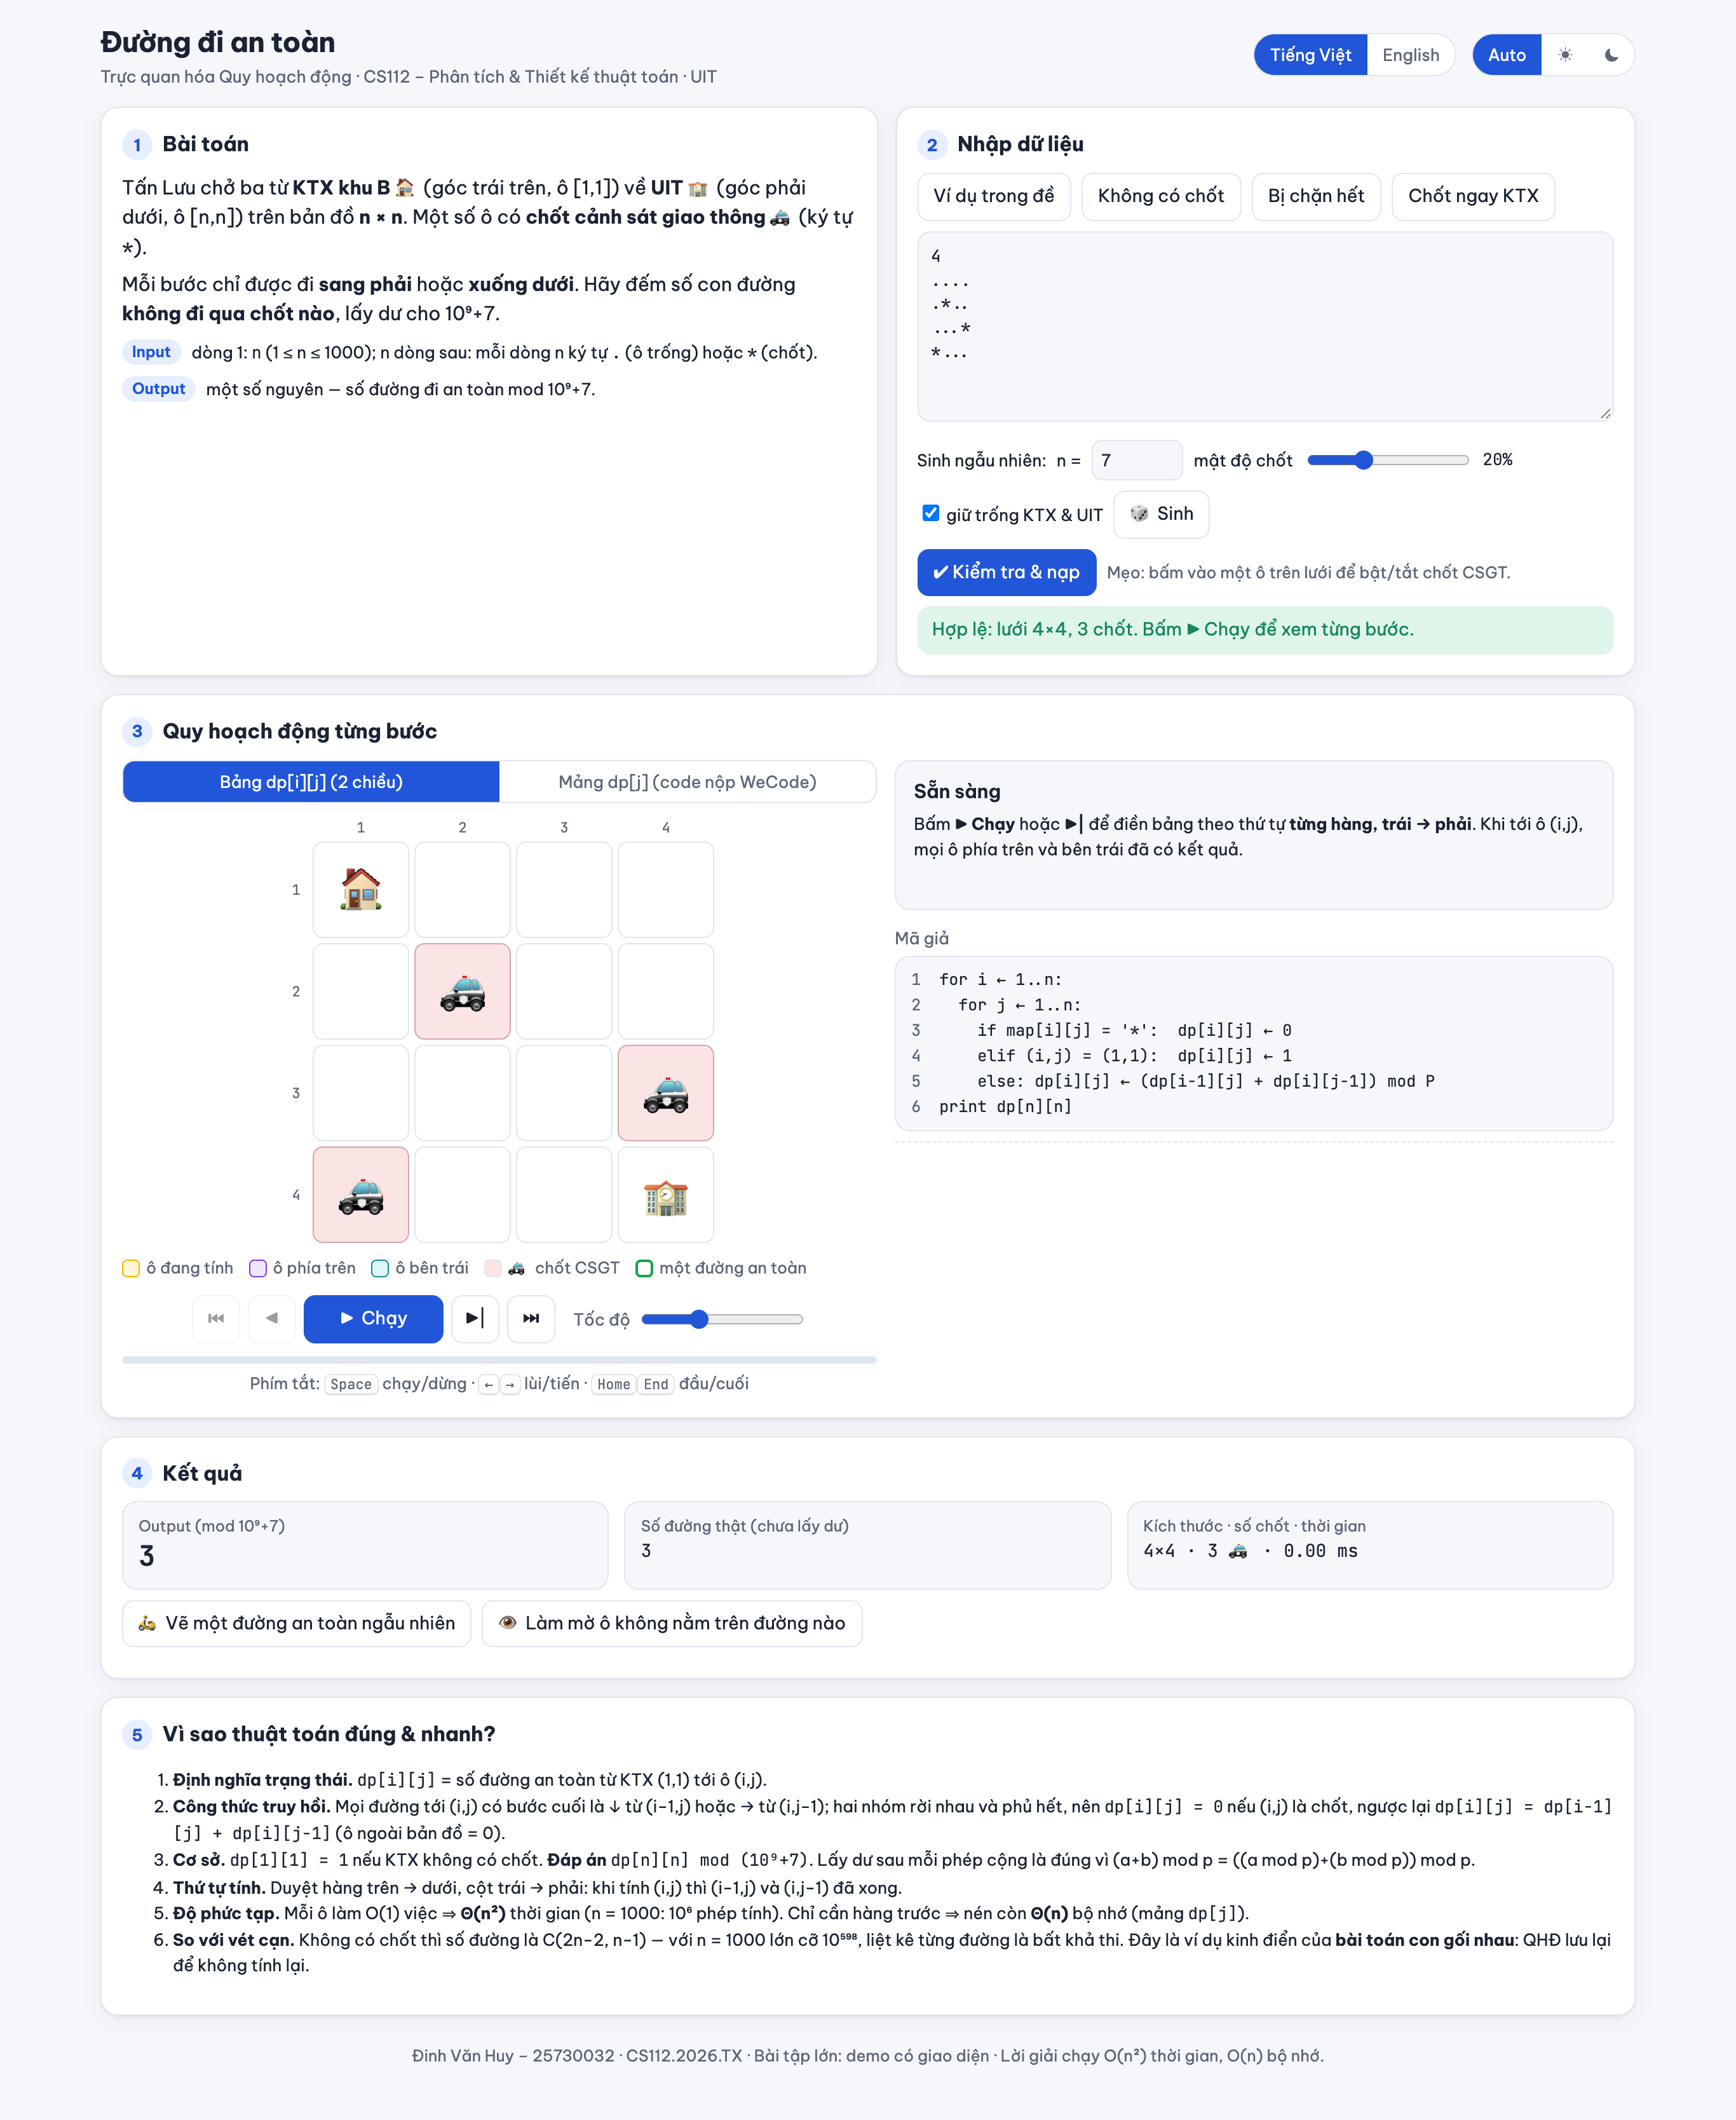
\includegraphics[width=\linewidth]{img/overview.png}
\caption{Toàn cảnh giao diện: đề bài, nhập dữ liệu, minh họa, kết quả, phân tích.}
\end{figure}
\begin{figure}[H]\centering
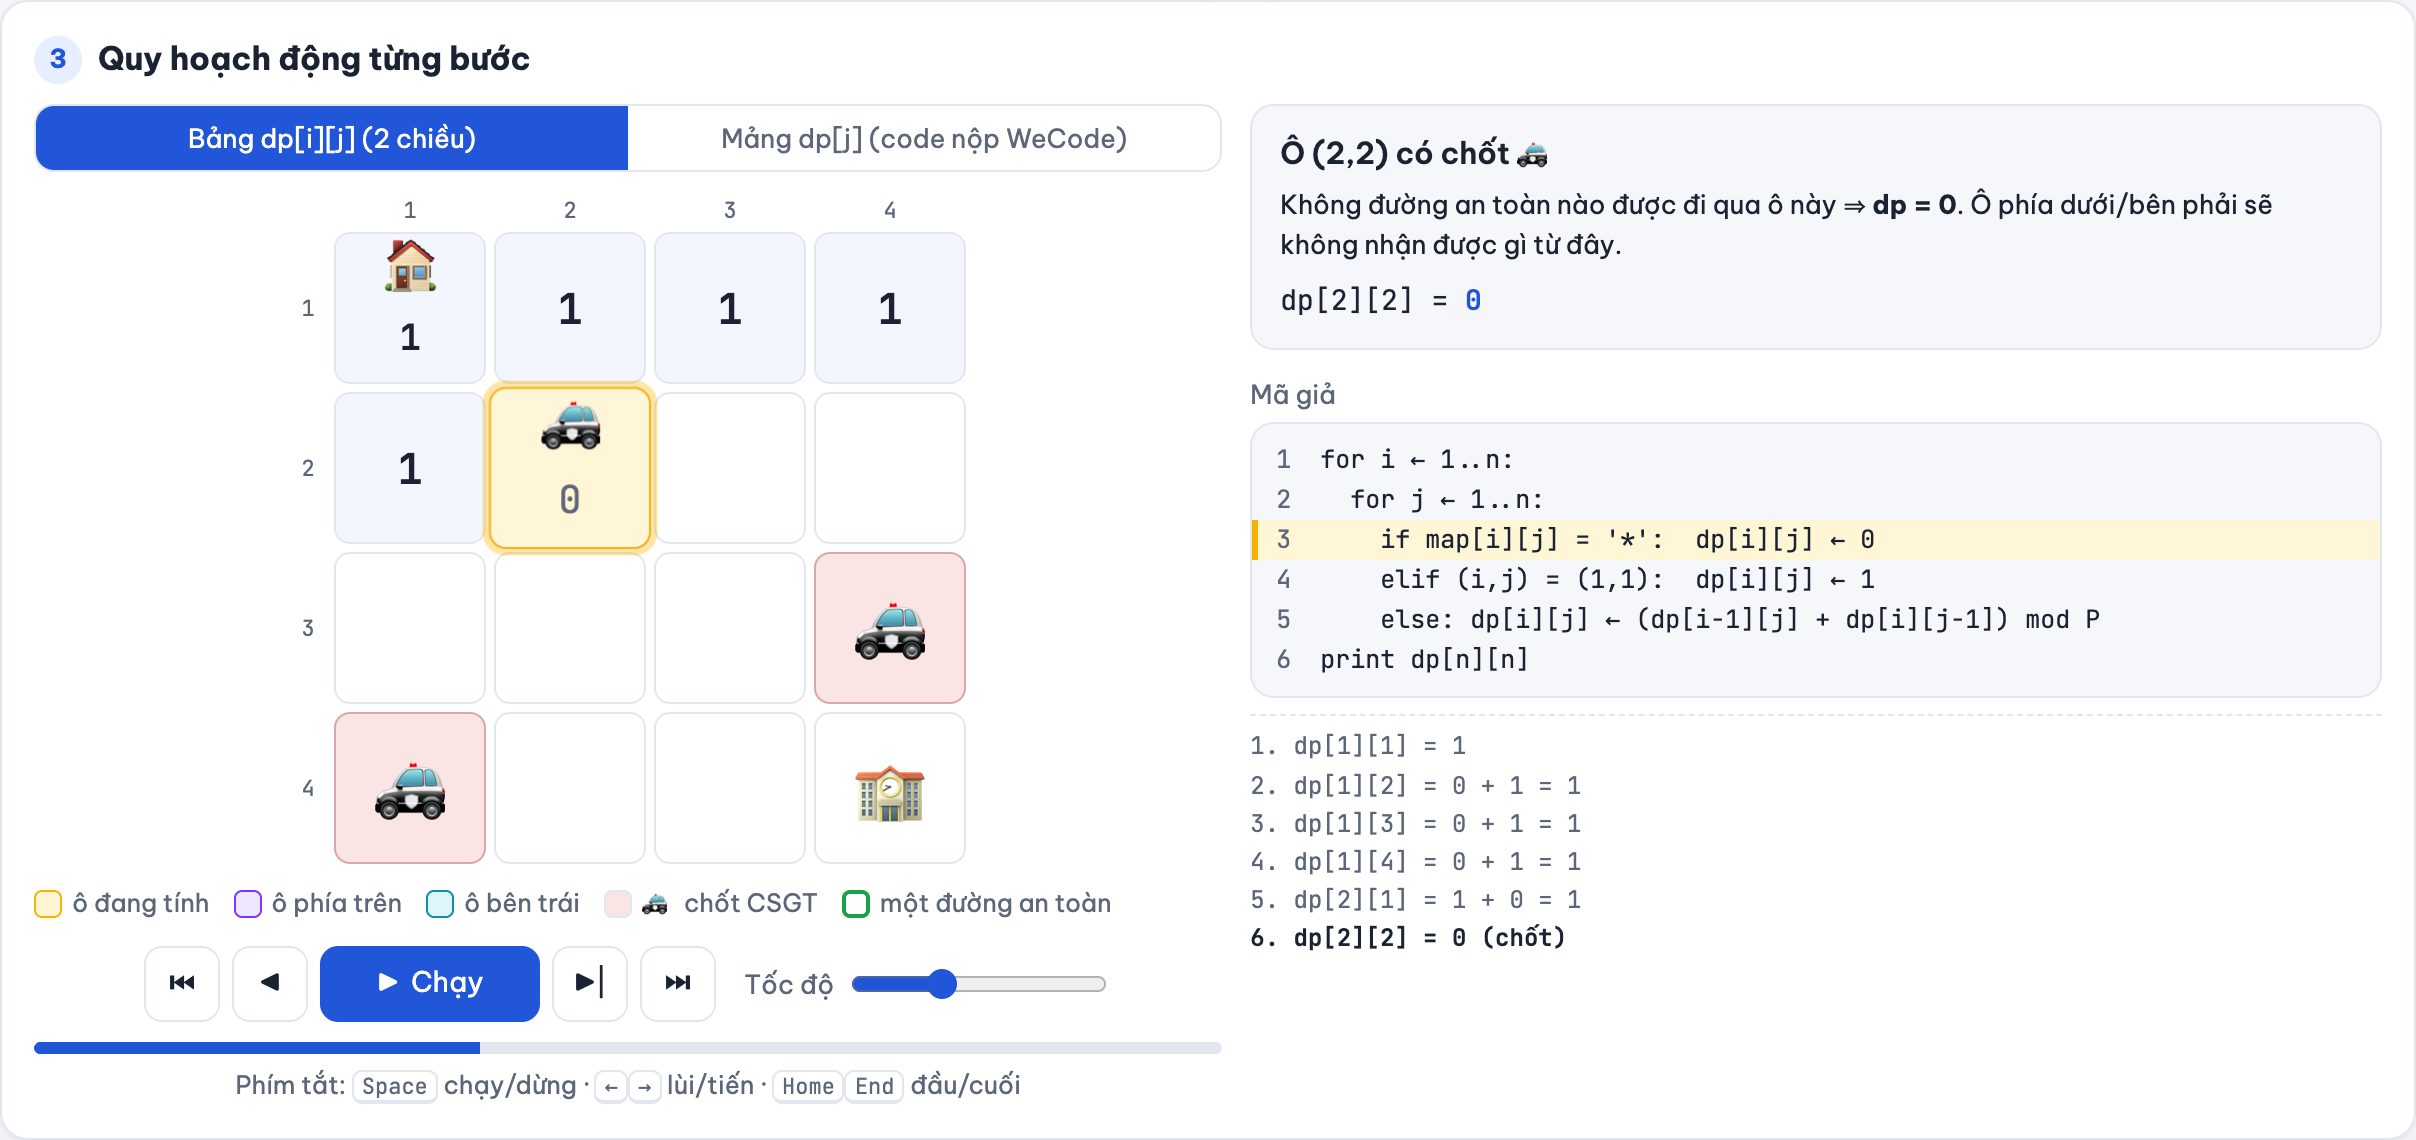
\includegraphics[width=\linewidth]{img/step_sum.png}
\caption{Bước tính một ô: cộng ô phía trên (tím) và ô bên trái (xanh); mã giả tô sáng dòng 5.}
\end{figure}
\begin{figure}[H]\centering
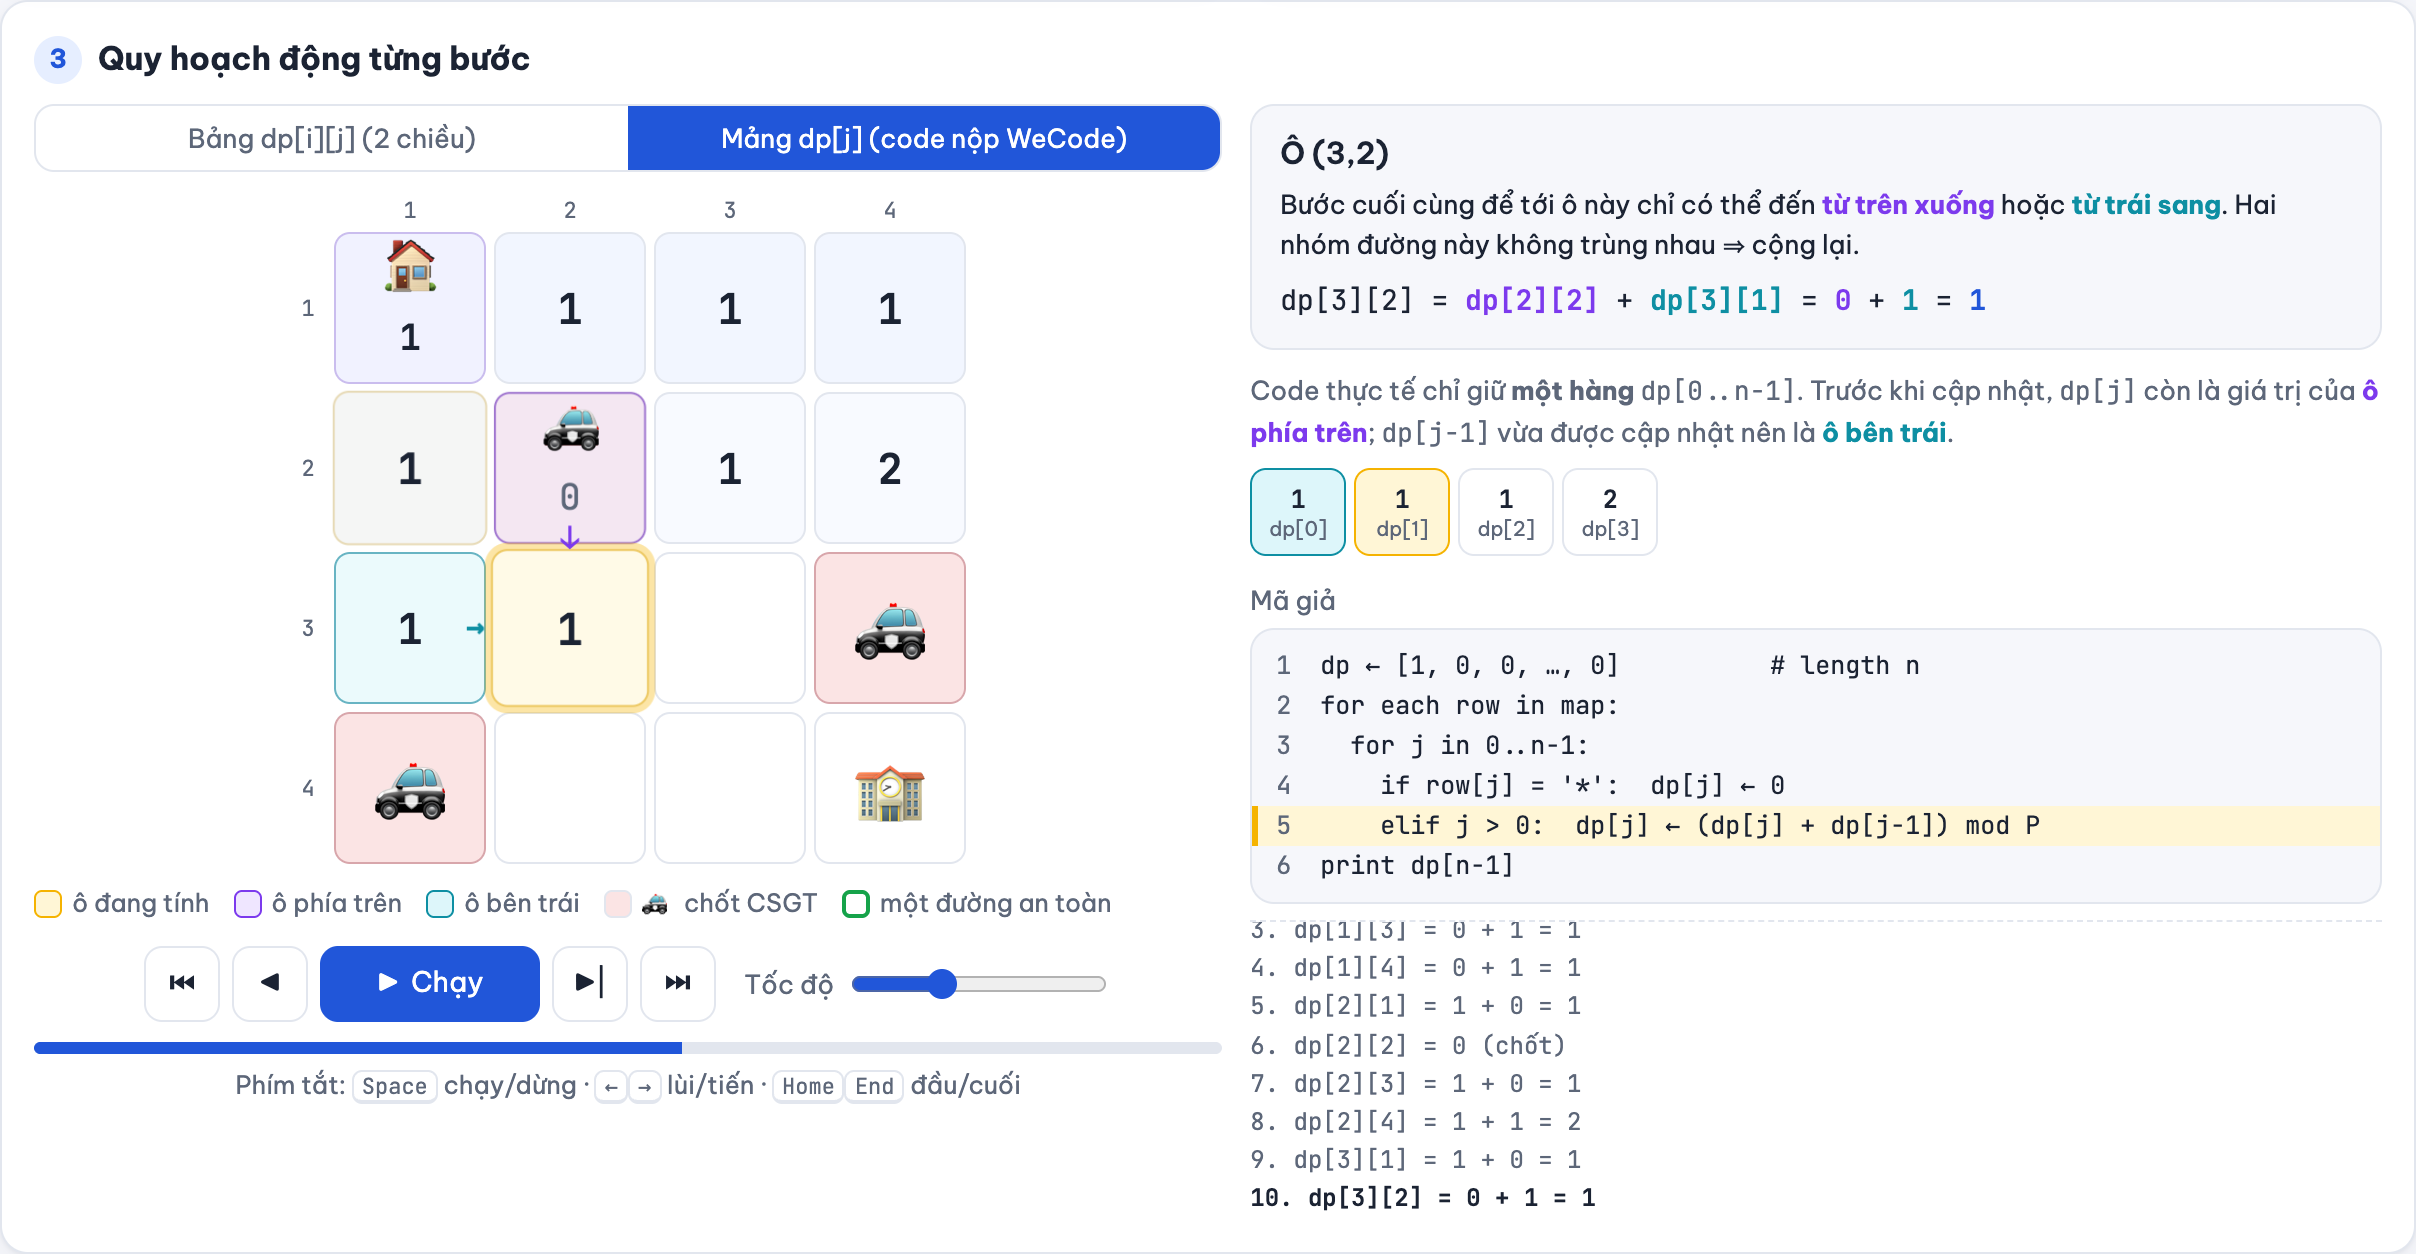
\includegraphics[width=\linewidth]{img/step_1d.png}
\caption{Chế độ mảng 1 chiều $dp[j]$ -- minh họa đúng code nộp WeCode.}
\end{figure}
\begin{figure}[H]\centering
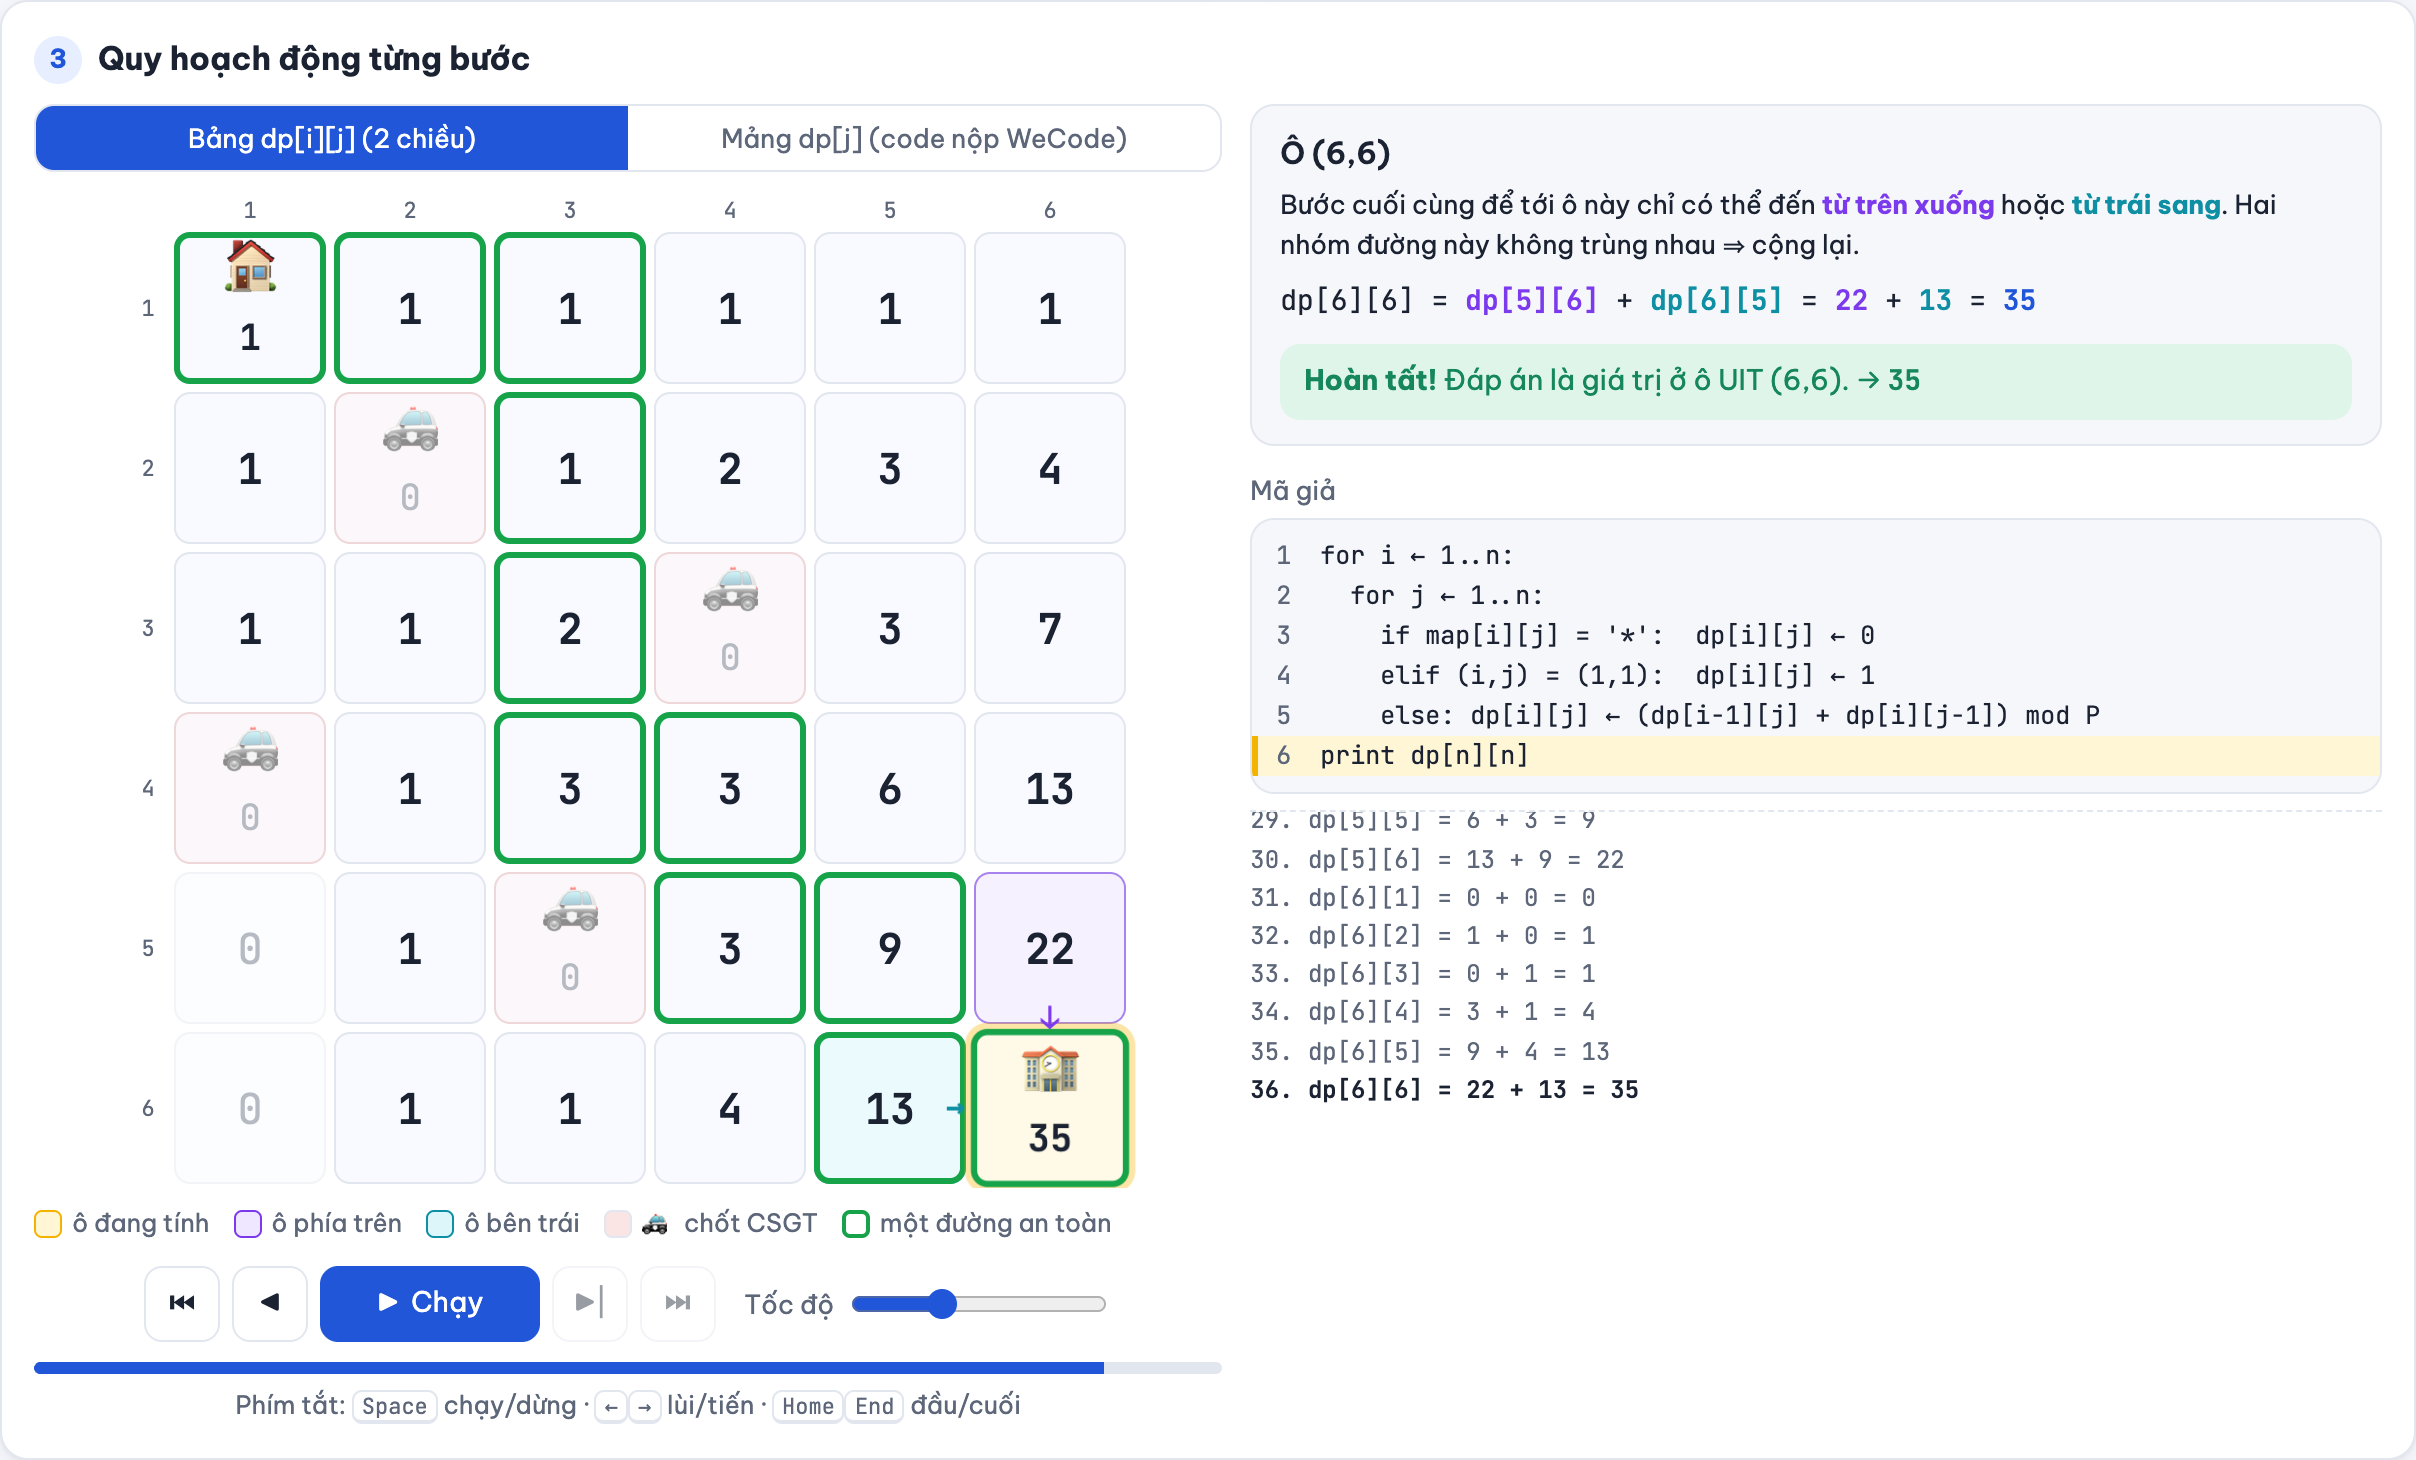
\includegraphics[width=\linewidth]{img/path.png}
\caption{Bản đồ $6\times6$ (35 đường): một đường an toàn ngẫu nhiên (viền xanh lá), các ô không nằm trên đường nào bị làm mờ.}
\end{figure}
\begin{figure}[H]\centering
\begin{minipage}{0.48\linewidth}\centering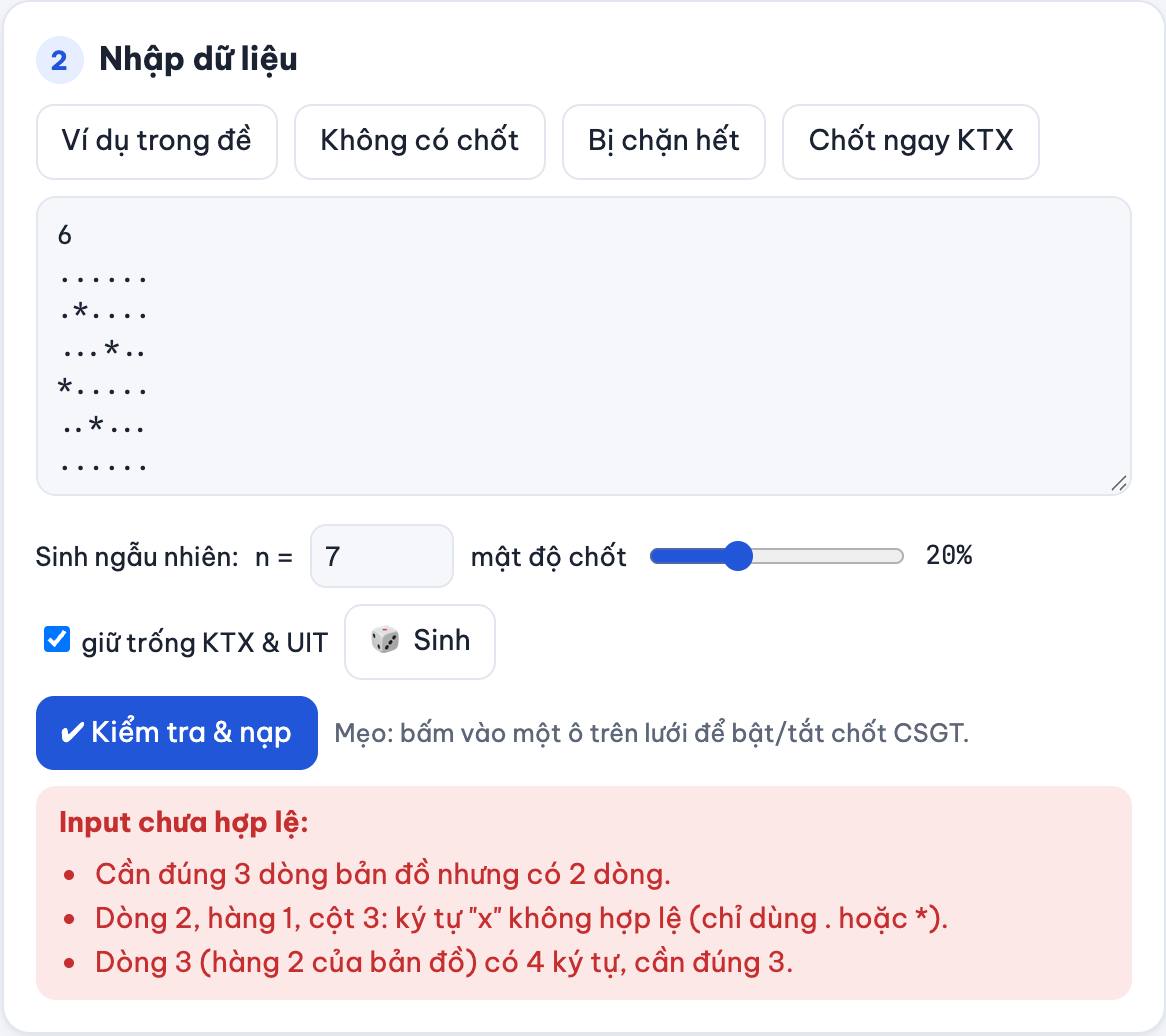
\includegraphics[width=\linewidth]{img/validate.png}\end{minipage}\hfill
\begin{minipage}{0.48\linewidth}\centering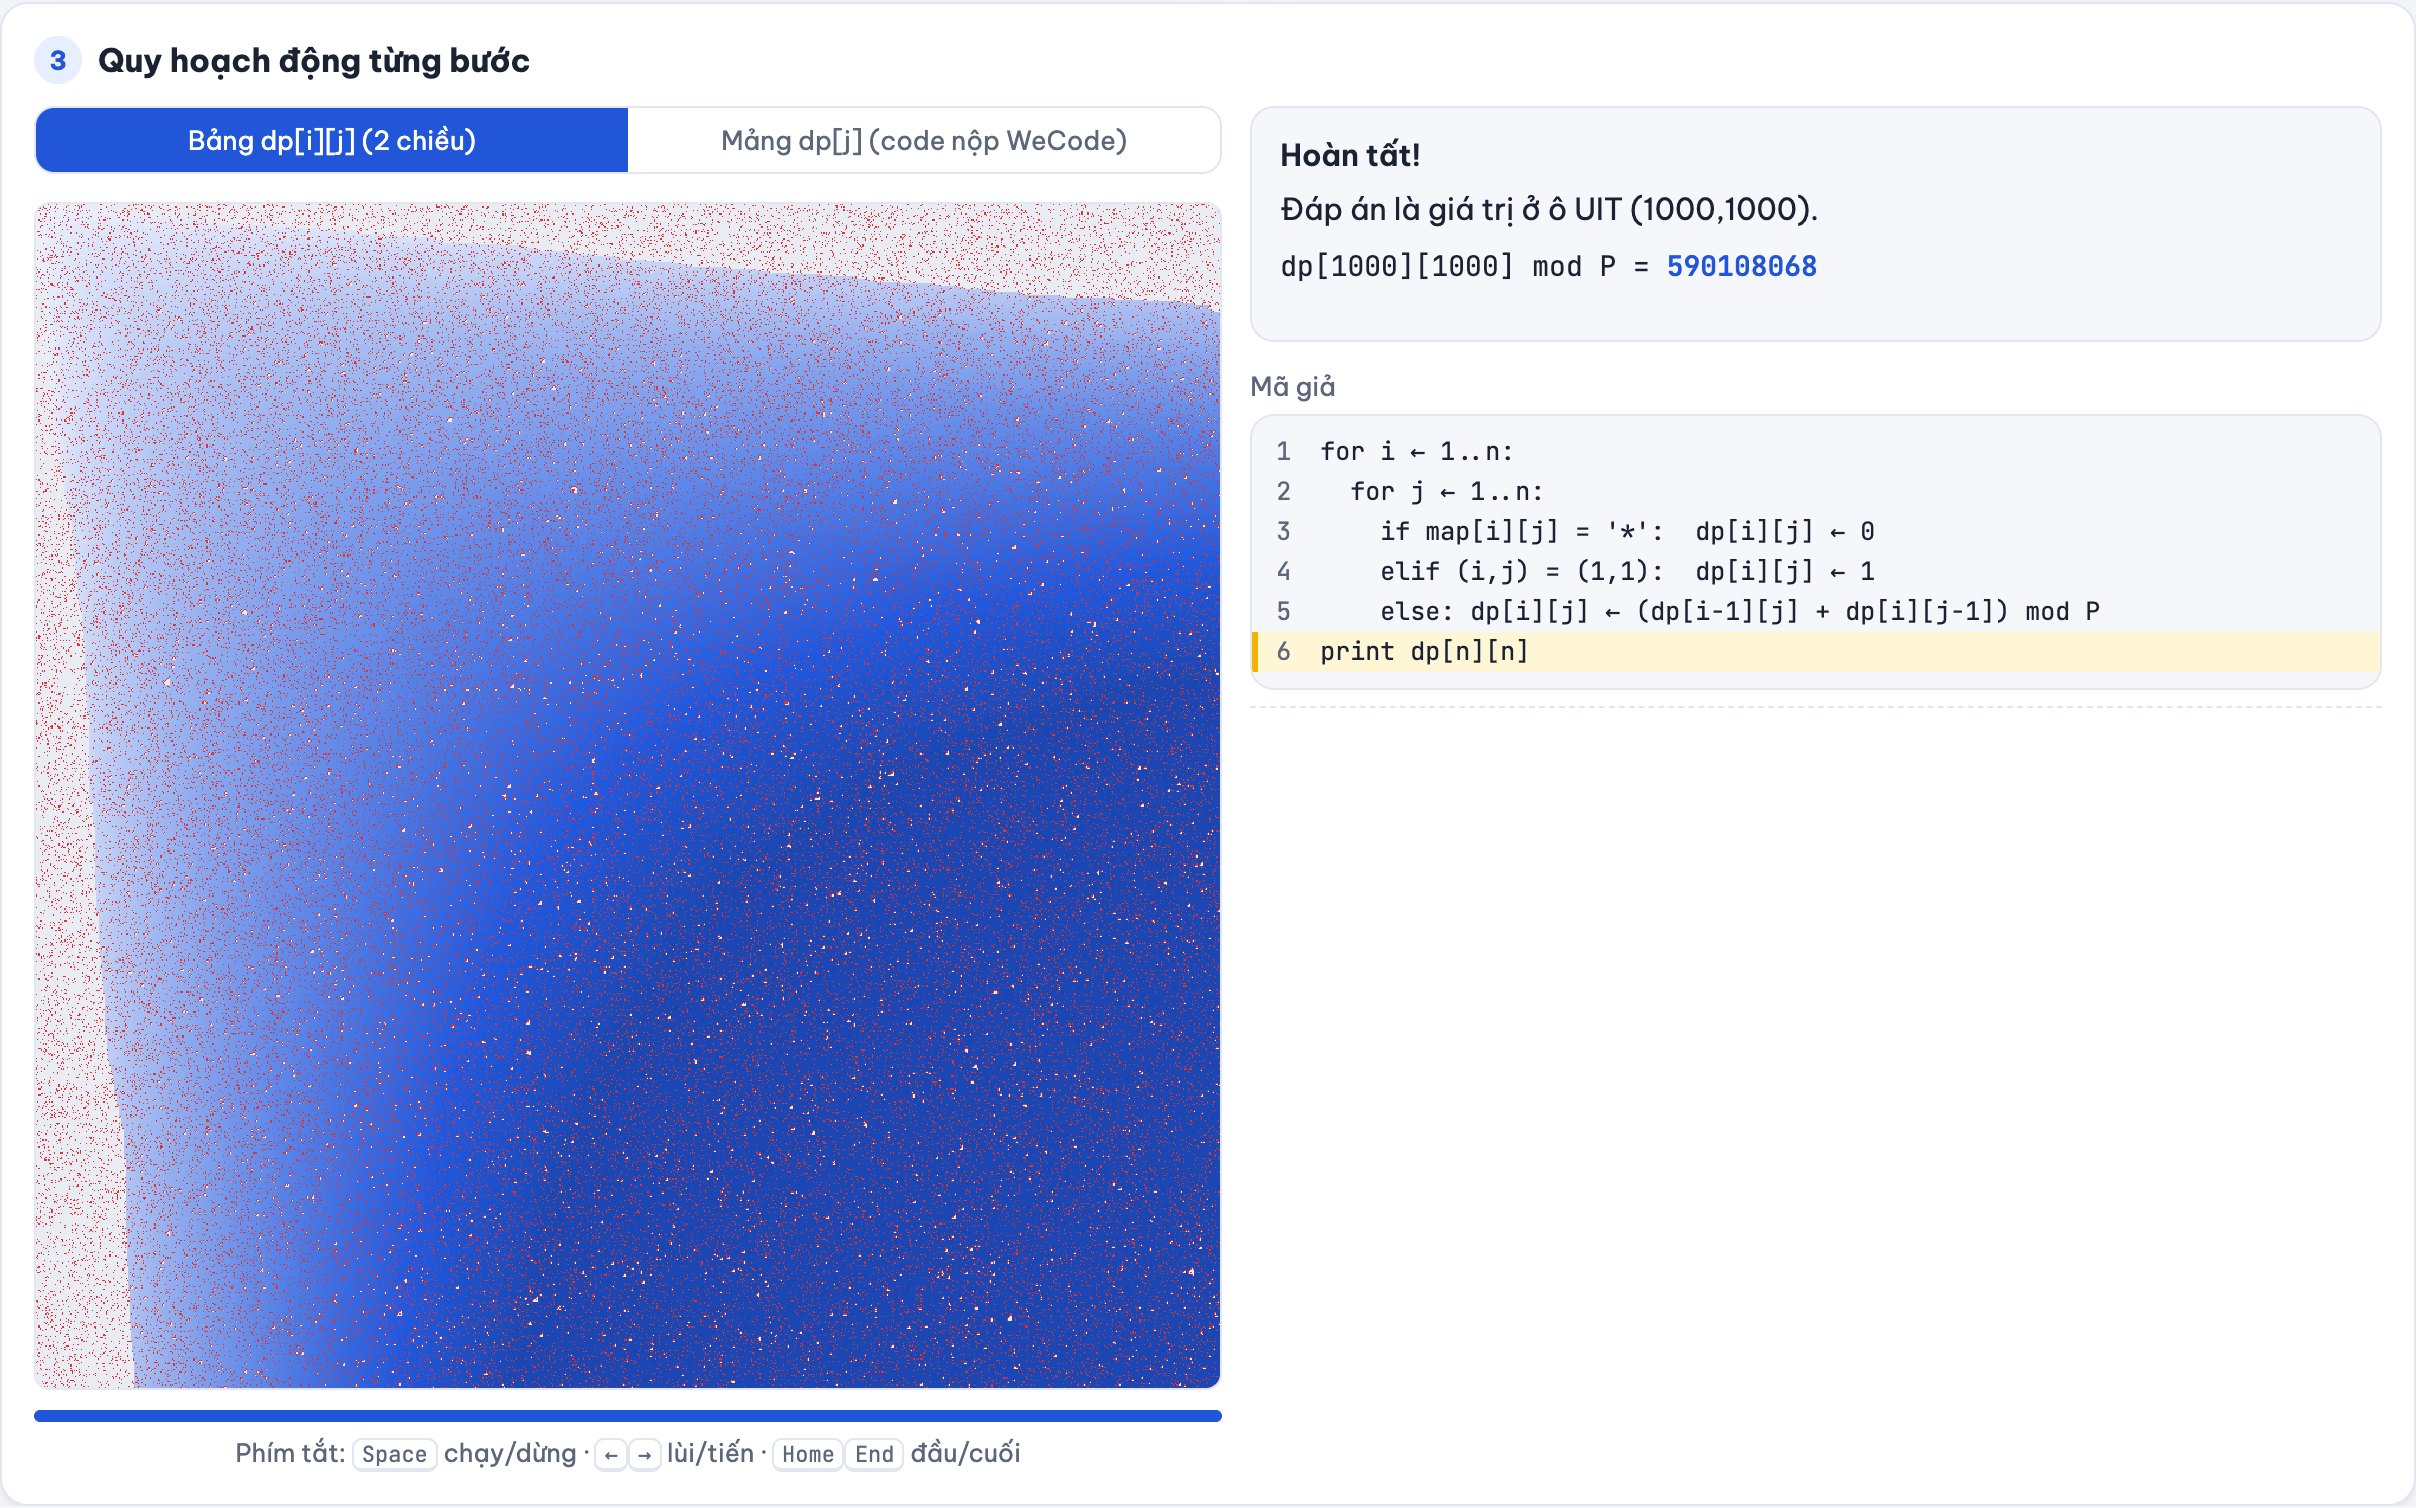
\includegraphics[width=\linewidth]{img/big.png}\end{minipage}
\caption{Trái: báo lỗi input kèm vị trí. Phải: lưới $1000\times1000$ hiển thị bằng bản đồ nhiệt.}
\end{figure}
\begin{figure}[H]\centering
\begin{minipage}{0.66\linewidth}\centering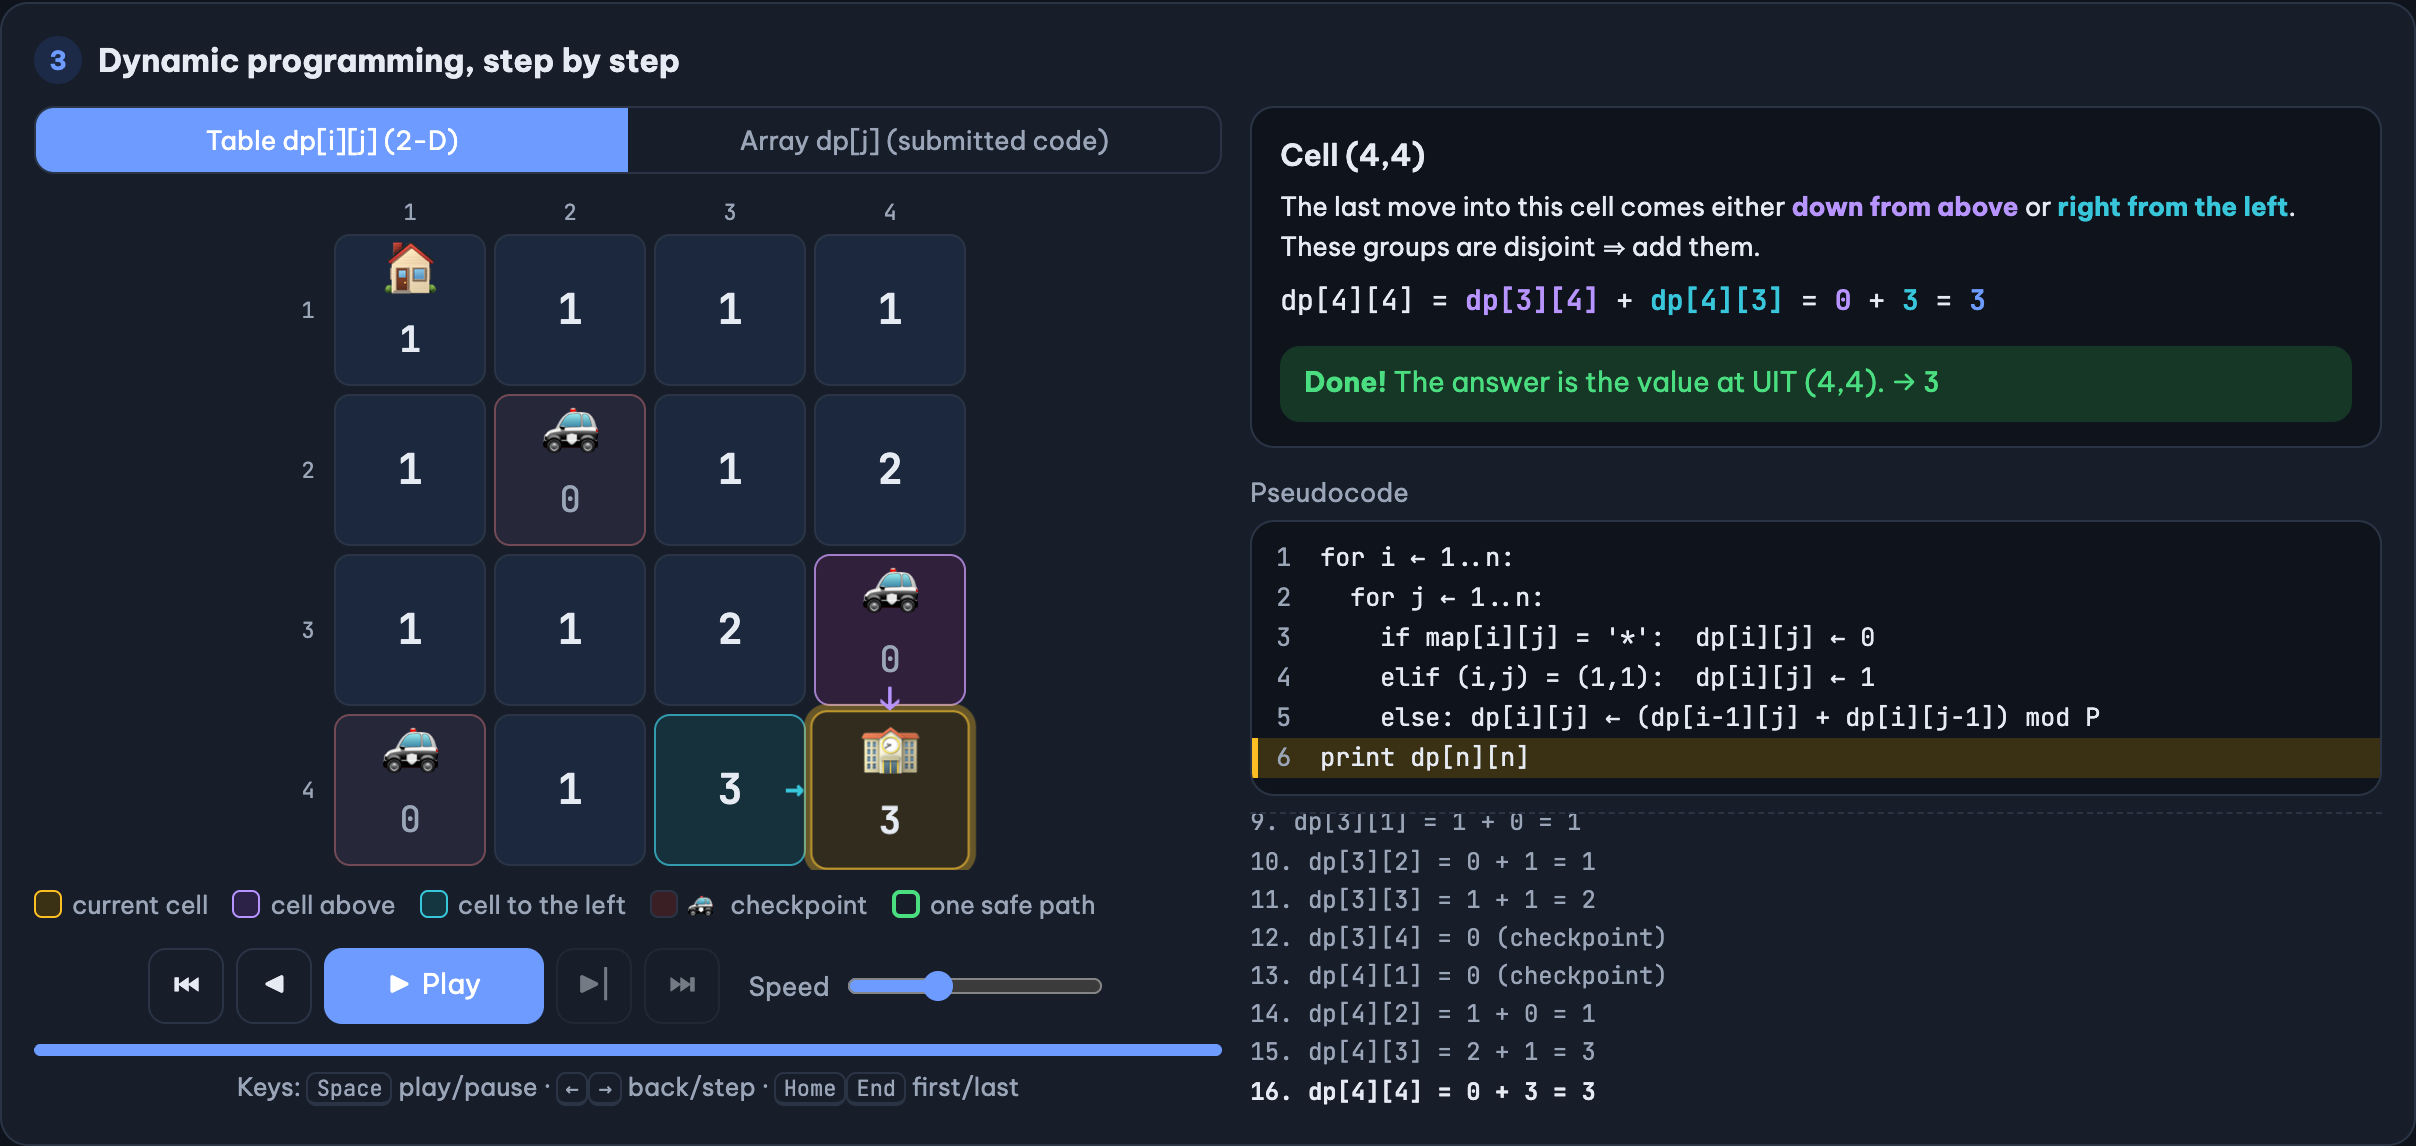
\includegraphics[width=\linewidth]{img/english_dark.png}\end{minipage}\hfill
\begin{minipage}{0.3\linewidth}\centering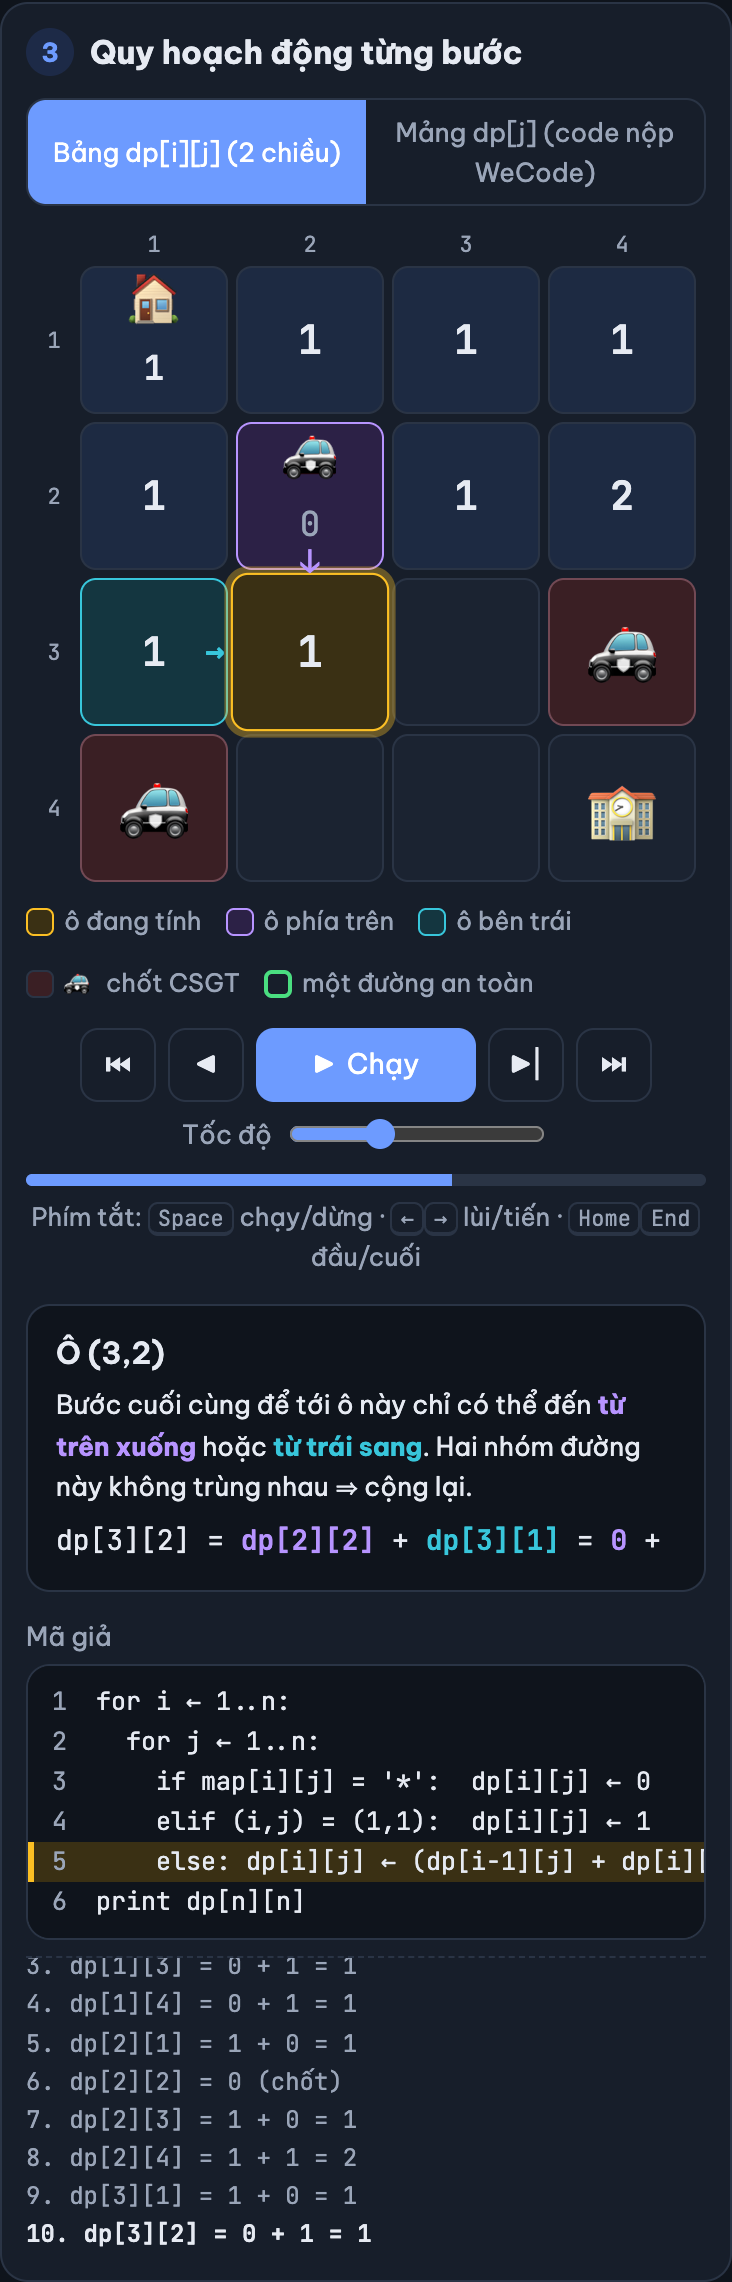
\includegraphics[width=\linewidth]{img/mobile.png}\end{minipage}
\caption{Giao diện tiếng Anh, nền tối (trái) và trên điện thoại (phải).}
\end{figure}

\subsection{Video demo}
Video \texttt{video/demo.mp4} (khoảng 3 phút, có thuyết minh tiếng Việt và phụ đề) được \textbf{tạo tự động} bằng script \texttt{video/make\_video.py}: Playwright điều khiển trình duyệt Chrome theo kịch bản 16 cảnh và ghi hình; lời thuyết minh được đọc bằng công cụ chuyển văn bản thành giọng nói \texttt{say} của macOS (giọng ``Linh''); ffmpeg ghép hình và tiếng. Cách làm này giúp video có thể tạo lại y hệt bất cứ lúc nào sau khi sửa giao diện.

% =====================================================
\section{Quy trình thực hiện và cách sử dụng AI}\label{sec:quytrinh}
\subsection{Công cụ}
\begin{itemize}
  \item \textbf{AI:} Claude Code (mô hình Claude Opus 5.5 của Anthropic), chạy trong ứng dụng Claude desktop, có quyền đọc/ghi file trong thư mục môn học và chạy lệnh trên máy.
  \item \textbf{Công cụ khác:} Python 3, Node.js, Playwright + Google Chrome (chụp ảnh, quay video), ffmpeg, \texttt{say} (macOS), Tectonic (biên dịch LaTeX).
\end{itemize}

\subsection{Các bước và prompt đã dùng}
Toàn bộ quá trình diễn ra trong \textbf{một phiên làm việc} với Claude Code. Dưới đây là các prompt của em (giữ nguyên văn, chỉ rút gọn phần dán dài) và việc AI đã làm sau mỗi prompt.

\begin{longtable}{>{\raggedright\arraybackslash}p{0.43\linewidth} >{\raggedright\arraybackslash}p{0.5\linewidth}}
\toprule
\textbf{Prompt của em} & \textbf{AI đã làm}\\\midrule\endhead
\textit{``check tài liệu trong docs đọc transcript và cho tôi biết ở buổi máy, mốc thời gian nào cô yêu cầu làm bài tập lớn, nội dung yêu cầu là gì''} &
Tìm trong 10 file phụ đề \texttt{.vtt} của các buổi học các từ khóa (``bài tập lớn'', ``đồ án'', ``deadline''\dots), xác định yêu cầu nằm ở Buổi 8, trích nội dung kèm mốc thời gian.\\\midrule
Dán bản tóm tắt yêu cầu em tự viết lại, hỏi \textit{``như vậy đúng chưa?''} &
Đối chiếu lại transcript, xác nhận các ý đúng, chỉ ra chỗ cần sửa: mốc thời gian cuối buổi, mục ``source code'' là suy luận do phụ đề tự động ghi sai, thiếu việc về nhà thứ hai (bài QHĐ trên WeCode).\\\midrule
\textit{``\dots dựa vào những dữ liệu trên, hãy đưa ra những câu hỏi để giúp bạn có thể làm bài tập này.''} &
Đặt 17 câu hỏi về: chọn bài, công nghệ, mức độ trực quan, report, video, hình thức nộp.\\\midrule
Trả lời 17 câu hỏi: dán đề bài ``Đường đi an toàn'' và hình minh họa, dán lời giải Python, chọn web (JS/Python), có deploy, minh họa từng bước cho người mới học, nhập tay + sinh ngẫu nhiên + validate đầy đủ, song ngữ, report LaTeX ghi trung thực, \textit{``AI đề xuất rồi bạn kiểm chứng''}, AI tự làm video, làm cá nhân, nộp trong tuần. &
Viết lõi thuật toán JS; viết bộ test đối chiếu vét cạn (mục 4) và chạy; xây giao diện web; tự mở trong trình duyệt để kiểm tra (desktop, điện thoại, tiếng Anh, lưới $1000\times1000$, input lỗi) và sửa các lỗi hiển thị phát hiện được; viết script quay video, phát hiện và khắc phục lỗi video bị hụt khung ở đáy; chụp ảnh và viết report này.\\
\bottomrule
\end{longtable}

\subsection{Phân định: phần nào do AI, phần nào do em}
\begin{itemize}
  \item \textbf{Chọn bài, yêu cầu sản phẩm} (đối tượng là người mới học, các chức năng cần có, song ngữ, hình thức report): em quyết định.
  \item \textbf{Thuật toán}: theo lựa chọn của em, \emph{AI đề xuất -- em kiểm chứng}. Công thức truy hồi, chứng minh và phân tích độ phức tạp ở mục 3 do AI trình bày; em kiểm chứng bằng chạy tay ví dụ trong đề, bằng bộ test đối chiếu vét cạn 307 trường hợp và test $n=1000$ so với công thức tổ hợp $\binom{1998}{999}$.
  \item \textbf{Code giao diện, script test, script video, report}: AI viết, em đọc lại, chạy thử và chỉnh sửa.
\end{itemize}

\begin{xacnhan}
\textbf{[Cần sinh viên điền/xác nhận trước khi nộp -- AI không biết các thông tin này]}
\begin{itemize}
  \item Nguồn gốc lời giải Python nộp WeCode (tự viết / tham khảo / dùng AI khác -- nếu có thì ghi rõ công cụ và prompt): \underline{\hspace{5cm}}
  \item Có tra cứu Google/tài liệu nào không (từ khóa, trang tham khảo): \underline{\hspace{5cm}}
  \item Những chỉnh sửa em tự làm thêm sau khi AI tạo sản phẩm: \underline{\hspace{5cm}}
\end{itemize}
\end{xacnhan}

\subsection{Nhận xét về việc dùng AI}
\begin{itemize}
  \item \textbf{Điểm mạnh:} AI làm rất nhanh phần ``tay chân'' (giao diện, kiểm thử, quay video) và tự kiểm tra sản phẩm trên trình duyệt, nhờ đó phát hiện được lỗi hiển thị (ô KTX bị che giá trị, khoảng trống thừa dưới lưới, tràn ngang trên điện thoại, video hụt khung).
  \item \textbf{Rủi ro:} AI có thể đưa ra lời giải sai nhưng trình bày rất thuyết phục. Vì vậy phần kiểm chứng độc lập (vét cạn, công thức tổ hợp) là bắt buộc chứ không chỉ tin vào lập luận.
  \item \textbf{Bài học:} Để dùng AI hiệu quả cần cung cấp đủ ngữ cảnh (đề bài, định dạng input, code hiện có, đối tượng người dùng). Việc AI hỏi lại 17 câu trước khi làm giúp sản phẩm đúng ý ngay từ đầu.
\end{itemize}

% =====================================================
\section{Đánh giá và hướng phát triển}
\textbf{Đã đạt:} đủ ba sản phẩm nộp; giao diện có nhập liệu, kiểm tra input, minh họa từng bước, giải thích công thức, chạy được tới $n=1000$; lời giải được kiểm chứng.\\
\textbf{Hạn chế:} hoạt hình từng ô chỉ áp dụng cho $n\le16$ để lưới còn đọc được; bản đồ nhiệt dùng số thực nên chỉ mang tính minh họa; giọng thuyết minh là giọng máy.\\
\textbf{Hướng phát triển:} so sánh trực quan với cách vét cạn (đếm số lời gọi đệ quy) để thấy rõ lợi ích của QHĐ; mở rộng cho phép đi theo 3 hướng, hoặc tìm đường an toàn có chi phí nhỏ nhất.

% =====================================================
\appendix
\section{Phụ lục: lời giải nộp WeCode (Python)}
\lstinputlisting[language=Python]{../solution/safe_path.py}

\section{Phụ lục: cấu trúc thư mục nộp}
\begin{lstlisting}[numbers=none]
DoAn_DuongDiAnToan/
  app/index.html, app/core.js   giao dien web + loi thuat toan
  solution/safe_path.py         loi giai nop WeCode
  tests/run_tests.py            doi chieu vet can, test lon, test validate
  video/demo.mp4                video demo (co thuyet minh)
  video/make_video.py           script tao video tu dong
  report/report.tex, report.pdf bao cao nay
\end{lstlisting}

\end{document}
